\documentclass[UTF8]{ctexart}
\usepackage{minted}
\usepackage{graphicx}
\usepackage{float}
\usepackage{subfigure}
\usepackage{geometry}
\geometry{a4paper, scale=0.8}
\title{Visual Odomentry代码阅读报告}
\author{唐誉铭}
\date{\today}
\begin{document}
	\maketitle
	\section{论文概要}
	\subsection{论文要解决的问题}
    论文中提出了一种基于双镜摄像头拍摄的视频进行三维重建的方法。3D感知是计算机视觉和机器人技术的核心课题之一。
    在实践中,相机的分辨率严重受限,并且对生成结果的准确性有着较高的要求。并且,该实时系统要求很高的计算性能
    ,很多嵌入式设备不能提供那么高的计算性能,特别是无法使用FPGA的情况下。

    论文中提到的处理方法实现了可以运行数千个特征点匹配的实时场景计算,一种简单而快速的视觉测距算法并且能推算出拍摄主体的自我运动。
    \subsection{论文采用的主要方法}
    在处理过程中,程序每次读入一帧左右两张图片,把图片加入ringbuffer中,并且用图1两种滤波器检测特征。
    \begin{figure}[H]
        \centering
        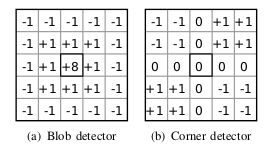
\includegraphics[width=0.6\textwidth]{img/filter.png} 
        \caption{采用的滤波器}
        \label{fig.1}
    \end{figure}
    分别求取结果较少的稀疏特征值和结果比较多的稠密特征值,并且分别用非极大值抑制和非极小值抑制处理得到的结果。

    下面的步骤是稀疏特征值匹配,首先对图像分成各个区域(bin)对每个特征点使用“环形匹配”,既先对于“前一帧”的左视图的每一个点,
    在“前一帧”右视图相似的位置找到对应的特征点,再找到该对应特征点在“当前帧”右视图对应的特征点,再寻找“当前帧”左视图对应的特征点,
    最后寻找“上一帧”左视图中的特征点对应的“当前帧”左视图对应的特征点。如果最后找到的特征点就是初始特征点,则“环形匹配”成功,否则失败。
    过程如图2,3所示。
    \begin{figure}[H]
        \centering
        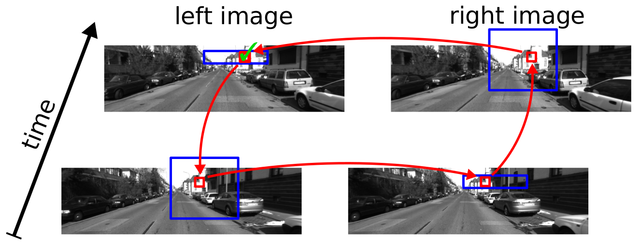
\includegraphics[width=0.75\textwidth]{img/CircleMatch.png}
        \caption{环形匹配过程}
        \label{fig.2}
    \end{figure}
    \begin{figure}[H]
        \centering
        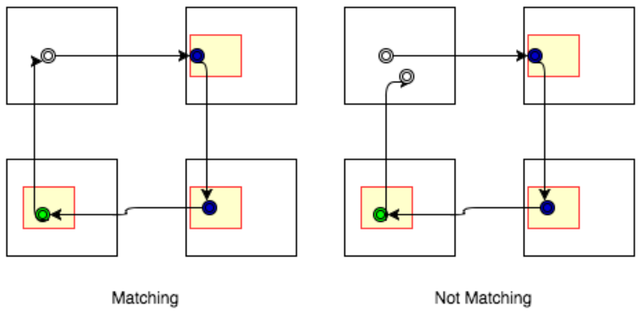
\includegraphics[width=0.75\textwidth]{img/CircleMatchOrNot.png}
        \caption{环形匹配是否成功}
        \label{fig.3}
    \end{figure}
    对匹配的结果使用2d Delaunay三角剖分来消去异常值,接下来对每一个匹配进行分析,统计每一个匹配完成的特征
    点在另外三张图的偏移距离大小,从而计算出每一个区域(bin)偏移范围,通过偏移范围确定下次稠密特征匹配的搜索范围。

    然后进行一次稠密点特征“环形匹配”,与稀疏特征匹配不同的是,后者的搜索范围是人工规定的比较大的区域
    ,而前者的搜索范围是由后者统计出偏移范围决定的。然后通过抛物线拟合的子像素细化来进一步改进特征定位,再使用三角剖分去除异常值。

    对匹配完成的结果再进行“桶”操作,把图像分为若干个桶,每个桶只随机保留若干个特征点,这样保证了特征点数量不会过多,并且较为
    均匀的分布在整个图像上。

    完成特征匹配后再进行动作推测。论文中提到的方法使用了RANSAC算法。在每轮RANSAC算法中,先随机选择3个点作为初始点,对这3个点建立动作预测模型,
    迭代求算出最优的位置调整参数,然后对所有特征点使用该动作预测模型,观测值与预测值只差小于某个阈值的特征点被标记为inlier,inlier越多代表
    模型越好,如果下一个模型的inlier数量比当前多,就更新模型。
	\section{代码分析}
    \subsection{主要类以及数据结构分析}
    \subsubsection{VisualOdometryStereo}
    主要功能类,包括动作预测,动作参数计算等功能
    \begin{minted}[linenos, breaklines, breakanywhere, mathescape]{c++}
class VisualOdometryStereo : public VisualOdometry {

public:

    struct parameters : public VisualOdometry::parameters {
        // 相关参数
        double  base;             // baseline (meters)
        int32_t ransac_iters;     // RANSAC迭代次数
        double  inlier_threshold; // inlier要求的偏差阈值
        bool    reweighting;      
    };

    bool process (uint8_t *I1,uint8_t *I2,int32_t* dims,bool replace=false);
    // 主要处理函数,读入两张照片

    using VisualOdometry::process;



private:

    std::vector<double>  estimateMotion (std::vector<Matcher::p_match> p_matched);
    // 预测动作
    enum                 result { UPDATED, FAILED, CONVERGED };  
    result               updateParameters(std::vector<Matcher::p_match> &p_matched,std::vector<int32_t> &active,std::vector<double> &tr,double step_size,double eps);
    // 更新动作变化参数
    void                 computeObservations(std::vector<Matcher::p_match> &p_matched,std::vector<int32_t> &active);
    void                 computeResidualsAndJacobian(std::vector<double> &tr,std::vector<int32_t> &active);
    // 计算相关参数
    std::vector<int32_t> getInlier(std::vector<Matcher::p_match> &p_matched,std::vector<double> &tr);
    // 计算inliers(内群点)

    double *X,*Y,*Z;    // 3d points
    double *p_residual; // residuals (p_residual=p_observe-p_predict)
    
    // parameters
    parameters param;
};
    \end{minted}
    \subsubsection{VisualOdometry}
    VisualOdometryStereo的基类
    \begin{minted}[linenos, breaklines, breakanywhere, mathescape]{c++}
class VisualOdometry {

public:

    // 镜头相关参数
    struct calibration {  
        double f;  // focal length (in pixels)
        double cu; // principal point (u-coordinate)
        double cv; // principal point (v-coordinate)
        calibration () {
            ...
        }
    };
    
    // “桶”操作参数
    struct bucketing {  
        int32_t max_features;  // maximal number of features per bucket 
        double  bucket_width;  // width of bucket
        double  bucket_height; // height of bucket
        bucketing () {
            ...
        }
    };
    
    // general parameters
    struct parameters {
        Matcher::parameters         match;            // matching parameters
        VisualOdometry::bucketing   bucket;           // bucketing parameters
        VisualOdometry::calibration calib;            // camera calibration parameters
    };


    // returns previous to current feature matches from internal matcher
    std::vector<Matcher::p_match> getMatches () { return matcher->getMatches(); }
    
    // streams out the current transformation matrix Tr_delta 
    friend std::ostream& operator<< (std::ostream &os,VisualOdometry &viso) {
        Matrix p = viso.getMotion();
        os << p.val[0][0] << " " << p.val[0][1] << " "  << p.val[0][2]  << " "  << p.val[0][3] << " ";
        os << p.val[1][0] << " " << p.val[1][1] << " "  << p.val[1][2]  << " "  << p.val[1][3] << " ";
        os << p.val[2][0] << " " << p.val[2][1] << " "  << p.val[2][2]  << " "  << p.val[2][3];
        return os;
    }
    
protected:

    // 更新动作
    bool updateMotion ();

    // 计算位置变化矩阵
    Matrix transformationVectorToMatrix (std::vector<double> tr);

    // 预测动作
    virtual std::vector<double> estimateMotion (std::vector<Matcher::p_match> p_matched) = 0;
    
    // 获得一个随机取样
    std::vector<int32_t> getRandomSample (int32_t N,int32_t num);

    Matrix                         Tr_delta;   // transformation (previous -> current frame)  
    bool                           Tr_valid;   // motion estimate exists?
    Matcher                       *matcher;    // feature matcher
    std::vector<int32_t>           inliers;    // inlier set
    double                        *J;          // jacobian
    double                        *p_observe;  // observed 2d points
    double                        *p_predict;  // predicted 2d points
    std::vector<Matcher::p_match>  p_matched;  // feature point matches
  
private:
  
    parameters                    param;     // common parameters
};
    \end{minted}
    \subsubsection{Matcher}
    提供维护一个ringbuffer,计算输入图片特征值,对特征值进行匹配,进行环形比配,对匹配结果进行桶操作,优化,去除无效值等
    特征计算以及匹配相关操作
    \begin{minted}[linenos, breaklines, breakanywhere, mathescape]{c++}
class Matcher {

public:

    // 各项参数
    struct parameters {
    
        int32_t nms_n;                  // non-max-suppression: min. distance between maxima (in pixels)
        int32_t nms_tau;                // non-max-suppression: interest point peakiness threshold
        int32_t match_binsize;          // matching bin width/height (affects efficiency only)
        int32_t match_radius;           // matching radius (du/dv in pixels)
        int32_t match_disp_tolerance;   // dv tolerance for stereo matches (in pixels)
        int32_t outlier_disp_tolerance; // outlier removal: disparity tolerance (in pixels)
        int32_t outlier_flow_tolerance; // outlier removal: flow tolerance (in pixels)
        int32_t multi_stage;            // 0=disabled,1=multistage matching (denser and faster)
        int32_t half_resolution;        // 0=disabled,1=match at half resolution, refine at full resolution
        int32_t refinement;             // refinement (0=none,1=pixel,2=subpixel)
        double  f,cu,cv,base;           // calibration (only for match prediction)
        
        parameters () {
            ...
        }
    };

    // 记录环形匹配完成后比配的四个点
    struct p_match {
        float   u1p,v1p; // u,v-coordinates in previous left  image
        int32_t i1p;     // feature index (for tracking)
        float   u2p,v2p; // u,v-coordinates in previous right image
        int32_t i2p;     // feature index (for tracking)
        float   u1c,v1c; // u,v-coordinates in current  left  image
        int32_t i1c;     // feature index (for tracking)
        float   u2c,v2c; // u,v-coordinates in current  right image
        int32_t i2c;     // feature index (for tracking)
    };

    // 读入一帧两张照片并且计算特征值
    void pushBack (uint8_t *I1,uint8_t* I2,int32_t* dims,const bool replace);
    
    // 匹配特征值
    void matchFeatures(int32_t method, Matrix *Tr_delta = 0);

    // 进行“桶”操作
    void bucketFeatures(int32_t max_features,float bucket_width,float bucket_height);

    // return vector with matched feature points and indices
    std::vector<Matcher::p_match> getMatches() { return p_matched_2; }

    private:

    // structure for storing interest points
    struct maximum {
        int32_t u;   // u-coordinate
        int32_t v;   // v-coordinate
        int32_t val; // value
        int32_t c;   // class
        int32_t d1,d2,d3,d4,d5,d6,d7,d8; // descriptor
        maximum() {}
        maximum(int32_t u,int32_t v,int32_t val,int32_t c):u(u),v(v),val(val),c(c) {}
    };
    
    // 记录统计出的搜索范围
    struct range {
        float u_min[4];
        float u_max[4];
        float v_min[4];
        float v_max[4];
    };
    
    // 统计每个匹配点位置在不同图中的变化值
    struct delta {
        float val[8];
        delta () {}
        delta (float v) {
        for (int32_t i=0; i<8; i++)
            val[i] = v;
        }
    };
    
    // 非极大值抑制
    void nonMaximumSuppression (int16_t* I_f1,int16_t* I_f2,const int32_t* dims,std::vector<Matcher::maximum> &maxima,int32_t nms_n);

    // descriptor functions
    inline uint8_t saturate(int16_t in);
    void filterImageAll (uint8_t* I,uint8_t* I_du,uint8_t* I_dv,int16_t* I_f1,int16_t* I_f2,const int* dims);
    void filterImageSobel (uint8_t* I,uint8_t* I_du,uint8_t* I_dv,const int* dims);
    inline void computeDescriptor (const uint8_t* I_du,const uint8_t* I_dv,const int32_t &bpl,const int32_t &u,const int32_t &v,uint8_t *desc_addr);
    inline void computeSmallDescriptor (const uint8_t* I_du,const uint8_t* I_dv,const int32_t &bpl,const int32_t &u,const int32_t &v,uint8_t *desc_addr);
    void computeDescriptors (uint8_t* I_du,uint8_t* I_dv,const int32_t bpl,std::vector<Matcher::maximum> &maxima);
    
    void getHalfResolutionDimensions(const int32_t *dims,int32_t *dims_half);
    uint8_t* createHalfResolutionImage(uint8_t *I,const int32_t* dims);

    // 计算图片特征
    void computeFeatures (uint8_t *I,const int32_t* dims,int32_t* &max1,int32_t &num1,int32_t* &max2,int32_t &num2,uint8_t* &I_du,uint8_t* &I_dv,uint8_t* &I_du_full,uint8_t* &I_dv_full);

    void computePriorStatistics (std::vector<Matcher::p_match> &p_matched,int32_t method);
    void createIndexVector (int32_t* m,int32_t n,std::vector<int32_t> *k,const int32_t &u_bin_num,const int32_t &v_bin_num);
    inline void findMatch (int32_t* m1,const int32_t &i1,int32_t* m2,const int32_t &step_size, std::vector<int32_t> *k2,const int32_t &u_bin_num,const int32_t &v_bin_num,const int32_t &stat_bin, int32_t& min_ind,int32_t stage,bool flow,bool use_prior,double u_=-1,double v_=-1);
    void matching (int32_t *m1p,int32_t *m2p,int32_t *m1c,int32_t *m2c, int32_t n1p,int32_t n2p,int32_t n1c,int32_t n2c, std::vector<Matcher::p_match> &p_matched,int32_t method,bool use_prior,Matrix *Tr_delta = 0);

    void removeOutliers (std::vector<Matcher::p_match> &p_matched,int32_t method);

    void refinement (std::vector<Matcher::p_match> &p_matched,int32_t method);

    // parameters
    parameters param;
    int32_t    margin;
    
    ...
};

    \end{minted}
    \subsection{主要函数过程分析}
    \subsubsection{demo程序分析}
    \begin{minted}[linenos, breaklines, breakanywhere, mathescape]{c++}
VisualOdometryStereo::parameters param;

// calibration parameters for sequence 2010_03_09_drive_0019 
param.calib.f  = 645.24; // focal length in pixels
param.calib.cu = 635.96; // principal point (u-coordinate) in pixels
param.calib.cv = 194.13; // principal point (v-coordinate) in pixels
param.base     = 0.5707; // baseline in meters
//新建一个参数,并且设置参数
// init visual odometry
VisualOdometryStereo viso(param);
//通过参数初始化一个VisualOdometryStereo实例
    \end{minted}
    新建参数并且初始化一个实例
    \begin{minted}[linenos, breaklines, breakanywhere, mathescape]{c++}
int32_t dims[] = {width,height,width};
if (viso.process(left_img_data,right_img_data,dims)) {

// on success, update current pose
pose = pose * Matrix::inv(viso.getMotion());

// output some statistics
double num_matches = viso.getNumberOfMatches();
double num_inliers = viso.getNumberOfInliers();
cout << ", Matches: " << num_matches;
cout << ", Inliers: " << 100.0*num_inliers/num_matches << " %" << ", Current pose: " << endl;
cout << pose << endl << endl;

} else {
cout << " ... failed!" << endl;
}
    \end{minted}
    分别从从左右镜头读入一帧,把图片中的信息存入数组,调用VisualOdemetryStereo的process方法进行处理,处理完成后输出匹配成功的点,内围点的占比和当前摄像机的姿态
    \subsubsection{VisualOdometryStereo::process}
    输入一帧左右两张图像,存入ringbuffer,计算特征,匹配特征值,进行“桶”操作,最后更新动作
    \begin{minted}[linenos, breaklines, breakanywhere, mathescape]{c++}
bool VisualOdometryStereo::process (uint8_t *I1,uint8_t *I2,int32_t* dims,bool replace) {

    matcher->pushBack(I1,I2,dims,replace);
    // 把左右两帧图片加入ringbuffer,并计算特征值
    
    // 如果是处理第一张图片就先建立动作预测
    if (!Tr_valid) {
        matcher->matchFeatures(2);
        matcher->bucketFeatures(param.bucket.max_features,param.bucket.bucket_width,param.bucket.bucket_height);                          
        p_matched = matcher->getMatches();
        updateMotion();
    }
    
    if (Tr_valid) matcher->matchFeatures(2,&Tr_delta);
    else          matcher->matchFeatures(2);
    // 使用环形匹配法匹配图像特征
    matcher->bucketFeatures(param.bucket.max_features,param.bucket.bucket_width,param.bucket.bucket_height);                          
    // 减少特征数量,并使特征值较为均匀的分布在图像中
    p_matched = matcher->getMatches();
    return updateMotion();
    // 更新动作
}
        
    \end{minted}
    \subsubsection{Matcher::pushBack} 
        把左右各一帧图像放入ringbuffer,并且计算两张图像的各个特征
    \begin{minted}[linenos, breaklines, breakanywhere, mathescape]{c++}
void Matcher::pushBack (uint8_t *I1,uint8_t* I2,int32_t* dims,const bool replace) {
    
    // 定义图片大小
    int32_t width  = dims[0];
    int32_t height = dims[1];
    int32_t bpl    = dims[2];

    // sanity check
    if (width<=0 || height<=0 || bpl<width || I1==0) {
        cerr << "ERROR: Image dimension mismatch!" << endl;
        return;
    }

    if (replace) {
        ... //如果规定了replace, 释放上上张图片的各项参数
    } else {
        ... //释放上上张图片的各项参数
        ... //将“当前”图片的各项信息设为“上张”图片的各项信息
    }

    // 对齐内存
    dims_c[0] = width;
    dims_c[1] = height;
    dims_c[2] = width + 15-(width-1)%16;

    I1c = (uint8_t*)_mm_malloc(dims_c[2]*dims_c[1]*sizeof(uint8_t),16);
    I2c = (uint8_t*)_mm_malloc(dims_c[2]*dims_c[1]*sizeof(uint8_t),16);
    ... // 对齐放置图片信息

    // 计算图片各项特征
    computeFeatures(I1c,dims_c,m1c1,n1c1,m1c2,n1c2,I1c_du,I1c_dv,I1c_du_full,I1c_dv_full);
    if (I2!=0)
        computeFeatures(I2c,dims_c,m2c1,n2c1,m2c2,n2c2,I2c_du,I2c_dv,I2c_du_full,I2c_dv_full);
    }
    \end{minted}
    \subsubsection{Matcher::computeFeatures}
    用各个滤波器提取图片的特征值,进行非极大化抑制,计算出稀疏特征以及稠密特征
    \begin{minted}[linenos, breaklines, breakanywhere, mathescape]{c++}
void Matcher::computeFeatures (...) {
  
    ...

    if (!param.half_resolution) {
        ... // demo不涉及这个部分
    } else {
        uint8_t* I_matching = createHalfResolutionImage(I,dims);
        getHalfResolutionDimensions(dims,dims_matching);
        // 将图像缩小一半
        ... // 为各个滤波结果分配空间
        filter::sobel5x5(I_matching,I_du,I_dv,dims_matching[2],dims_matching[1]);
        // 对缩略图进行sobel滤波求梯度
        filter::sobel5x5(I,I_du_full,I_dv_full,dims[2],dims[1]);
        // 对原图图进行sobel滤波求梯度
        filter::blob5x5(I_matching,I_f1,dims_matching[2],dims_matching[1]);
        // 对缩略图使用blob滤波
        filter::checkerboard5x5(I_matching,I_f2,dims_matching[2],dims_matching[1]);
        // 对缩略图求边界
        _mm_free(I_matching);
    }
    
    // 使用非极大抑制提取稀疏极大值
    vector<Matcher::maximum> maxima1;
    if (param.multi_stage) {
        int32_t nms_n_sparse = param.nms_n*3;
        if (nms_n_sparse>10)
            nms_n_sparse = max(param.nms_n,10);
        nonMaximumSuppression(I_f1,I_f2,dims_matching,maxima1,nms_n_sparse);
        computeDescriptors(I_du,I_dv,dims_matching[2],maxima1);
    }
    
    // 使用非极大抑制提取稠密极大值
    vector<Matcher::maximum> maxima2;
    nonMaximumSuppression(I_f1,I_f2,dims_matching,maxima2,param.nms_n);
    computeDescriptors(I_du,I_dv,dims_matching[2],maxima2);

    ...

    if (num1!=0) {
        ... // 将稀疏最大值对齐内存存入返回变量
    }
    
    if (num2!=0) {
        ... // 将稠密最大值对齐内存存入返回变量
    }
}

    \end{minted}
    \subsubsection{Matcher::matchFeatures}
    
    匹配特征值, 首先匹配稀疏特征值,消除异常值后计算出搜索范围,然后利用搜索范围进行稠密特征匹配,并且进行精化,消除异常值
    \begin{minted}[linenos, breaklines, breakanywhere, mathescape]{c++}
void Matcher::matchFeatures(int32_t method, Matrix *Tr_delta) {

    ... // 检查完整性

    // double pass matching
    if (param.multi_stage) {

        // 1st pass 稀疏特征匹配
        matching(m1p1,m2p1,m1c1,m2c1,n1p1,n2p1,n1c1,n2c1,p_matched_1,method,false,Tr_delta);
        // 使用2d Delaunay三角剖分消除异常值
        removeOutliers(p_matched_1,method);
        
        // 为加速第二次处理计算搜索范围优先级数据
        computePriorStatistics(p_matched_1,method);      

        // 2nd pass 稠密特征匹配
        matching(m1p2,m2p2,m1c2,m2c2,n1p2,n2p2,n1c2,n2c2,p_matched_2,method,true,Tr_delta);
        if (param.refinement>0)
            // 通过抛物线拟合的子像素细化来进一步改进特征定位
            refinement(p_matched_2,method);
        removeOutliers(p_matched_2,method);

    // single pass matching
    } else {
        ...
    }
}
    \end{minted}
    \subsubsection{Matcher::matching}
    对当前4张图片使用环形匹配
    \begin{minted}[linenos, breaklines, breakanywhere, mathescape]{c++}
void Matcher::matching (int32_t *m1p,int32_t *m2p,int32_t *m1c,int32_t *m2c, int32_t n1p,int32_t n2p,int32_t n1c,int32_t n2c, vector<Matcher::p_match> &p_matched,int32_t method,bool use_prior,Matrix *Tr_delta) {
    
    // loop variables
    int32_t* M = (int32_t*)calloc(dims_c[0]*dims_c[1],sizeof(int32_t));
    int32_t i1p,i2p,i1c,i2c,i1c2,i1p2;
    int32_t u1p,v1p,u2p,v2p,u1c,v1c,u2c,v2c;
    
    double t00,t01,t02,t03,t10,t11,t12,t13,t20,t21,t22,t23;
    if (Tr_delta) {
        ... // 如果存在之前的姿态变化量,就初始化变量
    }

    /////////////////////////////////////////////////////
    // method: flow
    if (method==0) {
        ... // demo不涉及这个部分
    }
        
    /////////////////////////////////////////////////////
    // method: stereo
    } else if (method==1) {
        ... // demo不涉及这个部分
    }
        
    /////////////////////////////////////////////////////
    // method: quad matching
    } else {
        
        // create position/class bin index vectors
        createIndexVector(m1p,n1p,k1p,u_bin_num,v_bin_num);
        createIndexVector(m2p,n2p,k2p,u_bin_num,v_bin_num);
        createIndexVector(m1c,n1c,k1c,u_bin_num,v_bin_num);
        createIndexVector(m2c,n2c,k2c,u_bin_num,v_bin_num);
        
        // for all points do
        for (i1p=0; i1p<n1p; i1p++) {
            // 对所有“前一帧”左边视图的所有特征点执行下面的操作

            // 读取每个特征点的坐标
            u1p = *(m1p+step_size*i1p+0);
            v1p = *(m1p+step_size*i1p+1);

            // compute row and column of statistics bin to which this observation belongs
            int32_t u_bin = min((int32_t)floor((float)u1p/(float)param.match_binsize),u_bin_num-1);
            int32_t v_bin = min((int32_t)floor((float)v1p/(float)param.match_binsize),v_bin_num-1);
            int32_t stat_bin = v_bin*u_bin_num+u_bin;

            // match in circle
            // 开始环形匹配
            findMatch(m1p,i1p,m2p,step_size,k2p,u_bin_num,v_bin_num,stat_bin,i2p, 0,false,use_prior);
            // 匹配“前一帧”左视图和“前一帧”右视图的稀疏特征

            u2p = *(m2p+step_size*i2p+0);
            v2p = *(m2p+step_size*i2p+1);

            if (Tr_delta) {
            
                double d = max((double)u1p-(double)u2p,1.0);
                double x1p = ((double)u1p-param.cu)*param.base/d;
                double y1p = ((double)v1p-param.cv)*param.base/d;
                double z1p = param.f*param.base/d;

                double x2c = t00*x1p + t01*y1p + t02*z1p + t03 - param.base;
                double y2c = t10*x1p + t11*y1p + t12*z1p + t13;
                double z2c = t20*x1p + t21*y1p + t22*z1p + t23;

                double u2c_ = param.f*x2c/z2c+param.cu;
                double v2c_ = param.f*y2c/z2c+param.cv;

                // 如果有之前运动矩阵,就沿用这个运动矩阵
                // 这里假设运动是连续的,运动的变化较小
                findMatch(m2p,i2p,m2c,step_size,k2c,u_bin_num,v_bin_num,stat_bin,i2c, 1,true ,use_prior,u2c_,v2c_);
            } else {
                findMatch(m2p,i2p,m2c,step_size,k2c,u_bin_num,v_bin_num,stat_bin,i2c, 1,true ,use_prior);
            }
            // 匹配“前一帧”右侧图像和“当前帧”右侧图像
            findMatch(m2c,i2c,m1c,step_size,k1c,u_bin_num,v_bin_num,stat_bin,i1c, 2,false,use_prior);
            // 匹配”当前帧“左侧图像和”当前帧“右侧图像
            if (Tr_delta)
                findMatch(m1c,i1c,m1p,step_size,k1p,u_bin_num,v_bin_num,stat_bin,i1p2,3,true ,use_prior,u1p,v1p);
            else
                findMatch(m1c,i1c,m1p,step_size,k1p,u_bin_num,v_bin_num,stat_bin,i1p2,3,true ,use_prior);
            // 匹配”当前帧“左侧图像和”前一帧“右侧图像
            if (i1p2==i1p) {

                u2c = *(m2c+step_size*i2c+0); v2c = *(m2c+step_size*i2c+1);
                u1c = *(m1c+step_size*i1c+0); v1c = *(m1c+step_size*i1c+1);
                if (u1p>=u2p && u1c>=u2c) {
                
                    // 如果匹配成功,就把匹配的结果放入p_match中
                    p_matched.push_back(Matcher::p_match(u1p,v1p,i1p,u2p,v2p,i2p,u1c,v1c,i1c,u2c,v2c,i2c));
                }
            }
        }
    }

    // free memory
    ...
}
    \end{minted}
    \subsubsection{Matcher::bucketFeatures}
    对匹配完成的结果进行“桶”操作,对每个局部区域只随机保留若干个特征点
    \begin{minted}[linenos, breaklines, breakanywhere, mathescape]{c++}
void Matcher::bucketFeatures(int32_t max_features,float bucket_width,float bucket_height) {

    // 找到”当前帧“左侧图像u-v坐标做大的特征点
    float u_max = 0;
    float v_max = 0;
    for (vector<p_match>::iterator it = p_matched_2.begin(); it!=p_matched_2.end(); it++) {
        if (it->u1c>u_max) u_max=it->u1c;
        if (it->v1c>v_max) v_max=it->v1c;
    }

    // 分配需要的buckets
    int32_t bucket_cols = (int32_t)floor(u_max/bucket_width)+1;
    int32_t bucket_rows = (int32_t)floor(v_max/bucket_height)+1;
    vector<p_match> *buckets = new vector<p_match>[bucket_cols*bucket_rows];

    // 把每个特征点放入其位置对应的bukect中
    for (vector<p_match>::iterator it=p_matched_2.begin(); it!=p_matched_2.end(); it++) {
        int32_t u = (int32_t)floor(it->u1c/bucket_width);
        int32_t v = (int32_t)floor(it->v1c/bucket_height);
        buckets[v*bucket_cols+u].push_back(*it);
    }
    
    p_matched_2.clear();
    // 清空原特征点
    for (int32_t i=0; i<bucket_cols*bucket_rows; i++) {
        // 对每个bucket
        
        std::random_shuffle(buckets[i].begin(),buckets[i].end());
        
        // 每个bucket随机填入max_features个特征点
        int32_t k=0;
        for (vector<p_match>::iterator it=buckets[i].begin(); it!=buckets[i].end(); it++) {
            p_matched_2.push_back(*it);
            k++;
            if (k>=max_features)
                break;
        }
    }

    // free buckets
    delete []buckets;
}        
    \end{minted}
    \subsubsection{Matcher::computePriorStatistics}
    分析偏移结果,统计每个区域最大偏移量,为下一部稠密特征匹配约束搜索范围
    \begin{minted}[linenos, breaklines, breakanywhere, mathescape]{c++}
void Matcher::computePriorStatistics (vector<Matcher::p_match> &p_matched,int32_t method) {
    
    // 计算区域(bin)数量
    int32_t u_bin_num = (int32_t)ceil((float)dims_c[0]/(float)param.match_binsize);
    int32_t v_bin_num = (int32_t)ceil((float)dims_c[1]/(float)param.match_binsize);
    int32_t bin_num   = v_bin_num*u_bin_num;
    
    ...

    for (vector<Matcher::p_match>::iterator it=p_matched.begin(); it!=p_matched.end(); it++) {
        // 对每一组配对好的点组
        // method flow: compute position delta
        if (method==0) {
            ... 
        } else if (method==1) {
            ... 
        } else {
            delta_curr.val[0] = it->u2p - it->u1p;
            delta_curr.val[1] = 0;
            delta_curr.val[2] = it->u2c - it->u2p;
            delta_curr.val[3] = it->v2c - it->v2p;
            delta_curr.val[4] = it->u1c - it->u2c;
            delta_curr.val[5] = 0;
            delta_curr.val[6] = it->u1p - it->u1c;
            delta_curr.val[7] = it->v1p - it->v1c;
            // 计算这个点组的各个偏移量
        }
        
        // 计算哪些区域(bin)包含了这个点组
        int32_t u_bin_min,u_bin_max,v_bin_min,v_bin_max;

        // flow + stereo: use current left image as reference
        if (method<2) {
            ...
        
        } else {
            u_bin_min = min(max((int32_t)floor(it->u1p/(float)param.match_binsize)-1,0),u_bin_num-1);
            u_bin_max = min(max((int32_t)floor(it->u1p/(float)param.match_binsize)+1,0),u_bin_num-1);
            v_bin_min = min(max((int32_t)floor(it->v1p/(float)param.match_binsize)-1,0),v_bin_num-1);
            v_bin_max = min(max((int32_t)floor(it->v1p/(float)param.match_binsize)+1,0),v_bin_num-1);
        }
        
        // 在相关区域对应的accumulator中加入计算出的偏移量
        for (int32_t v_bin=v_bin_min; v_bin<=v_bin_max; v_bin++)
            for (int32_t u_bin=u_bin_min; u_bin<=u_bin_max; u_bin++)
                delta_accu[v_bin*u_bin_num+u_bin].push_back(delta_curr);
    }
    
    ranges.clear();
    
    // 对每个区域(bin)计算最大偏移量
    for (int32_t v_bin=0; v_bin<v_bin_num; v_bin++) {
        for (int32_t u_bin=0; u_bin<u_bin_num; u_bin++) {
            
            // 如果此区域(bin)没有相关记录,就使用默认值
            delta delta_min(-param.match_radius);
            delta delta_max(+param.match_radius);
            
            // 通过每个区域(bin)的accumulator中的各个偏移值计算出最大偏移值
            if (delta_accu[v_bin*u_bin_num+u_bin].size()>0) {
                
                // init displacements 'delta' to 'infinite'
                delta_min = delta(+1000000);
                delta_max = delta(-1000000);
                
                // find minimum and maximum displacements
                for (vector<Matcher::delta>::iterator it=delta_accu[v_bin*u_bin_num+u_bin].begin();
                    it!=delta_accu[v_bin*u_bin_num+u_bin].end(); it++) {
                    for (int32_t i=0; i<num_stages*2; i++) {
                        if (it->val[i]<delta_min.val[i]) delta_min.val[i] = it->val[i];
                        if (it->val[i]>delta_max.val[i]) delta_max.val[i] = it->val[i];
                    }
                }
            }
        
            // 将最大偏移值进一步处理为搜索范围
            range r;
            for (int32_t i=0; i<num_stages; i++) {
                
                // bound minimum search range to 20x20
                float delta_u = delta_max.val[i*2+0]-delta_min.val[i*2+0];
                if (delta_u<20) {
                    delta_min.val[i*2+0] -= ceil((20-delta_u)/2);
                    delta_max.val[i*2+0] += ceil((20-delta_u)/2);
                }
                float delta_v = delta_max.val[i*2+1]-delta_min.val[i*2+1];
                if (delta_v<20) {
                    delta_min.val[i*2+1] -= ceil((20-delta_v)/2);
                    delta_max.val[i*2+1] += ceil((20-delta_v)/2);
                }
                
                // set range for this bin
                r.u_min[i] = delta_min.val[i*2+0];
                r.u_max[i] = delta_max.val[i*2+0];
                r.v_min[i] = delta_min.val[i*2+1];
                r.v_max[i] = delta_max.val[i*2+1];
            }
            ranges.push_back(r);      
        }
    }
    
    // free bin accumulator memory
    delete []delta_accu;
}
    \end{minted}
    \subsubsection{VisualOdometry::updateMotion}
    计算主体动作,并将其转换为矩阵
    \begin{minted}[linenos, breaklines, breakanywhere, mathescape]{c++}
bool VisualOdometry::updateMotion () {
  
  // 调用estimateMotion预测当前姿态变换
  vector<double> tr_delta = estimateMotion(p_matched);
  
  // on failure
  if (tr_delta.size()!=6)
    return false;
  
  // set transformation matrix (previous to current frame)
  Tr_delta = transformationVectorToMatrix(tr_delta);
  Tr_valid = true;
  
  // success
  return true;
}
    \end{minted}
    \subsubsection{VisualOdometryStereo::estimateMotion}
    使用RANSAC算法计算最优的投影参数
    \begin{minted}[linenos, breaklines, breakanywhere, mathescape]{c++}
vector<double> VisualOdometryStereo::estimateMotion (vector<Matcher::p_match> p_matched) {

    // compute minimum distance for RANSAC samples
    double width=0,height=0;
    for (vector<Matcher::p_match>::iterator it=p_matched.begin(); it!=p_matched.end(); it++) {
        if (it->u1c>width)  width  = it->u1c;
        if (it->v1c>height) height = it->v1c;
    }
    double min_dist = min(width,height)/3.0;
    
    // get number of matches
    int32_t N  = p_matched.size();
    if (N<6)
        return vector<double>();

    // allocate dynamic memory
    ...

    // project matches of previous image into 3d
    // 把之前一帧的匹配点投影在3D坐标内
    /* 
    $d$代表水平视差, $B$代表baseline(水平基线)
    $d=max(u_l-u_r, 0.0001)$
    $Z=\frac{f\times B}{d}$
    $X=(u-c_u)\frac{B}{d}$
    $Y=(v-c_v)\frac{B}{d}$
    */
    for (int32_t i=0; i<N; i++) {
        double d = max(p_matched[i].u1p - p_matched[i].u2p,0.0001f);
        X[i] = (p_matched[i].u1p-param.calib.cu)*param.base/d;
        Y[i] = (p_matched[i].v1p-param.calib.cv)*param.base/d;
        Z[i] = param.calib.f*param.base/d;
    }

    // loop variables
    vector<double> tr_delta;
    vector<double> tr_delta_curr;
    tr_delta_curr.resize(6);
    
    // clear parameter vector
    inliers.clear();

    // 进行ransac_iters轮RANSAC算法匹配
    for (int32_t k=0;k<param.ransac_iters;k++) {

        // 随机选择3个观测点作为初始inlier
        vector<int32_t> active = getRandomSample(N,3);

        // clear parameter vector
        for (int32_t i=0; i<6; i++)
        tr_delta_curr[i] = 0;

        // minimize reprojection errors
        VisualOdometryStereo::result result = UPDATED;
        int32_t iter=0;
        // 迭代寻找到最优的投影参数
        while (result==UPDATED) {
            result = updateParameters(p_matched,active,tr_delta_curr,1,1e-6);
            if (iter++ > 20 || result==CONVERGED)
                break; //迭代20次或者结果收敛就停止迭代
        }

        // overwrite best parameters if we have more inliers
        if (result!=FAILED) {
            vector<int32_t> inliers_curr = getInlier(p_matched,tr_delta_curr);
            // 获取符合当前模型的内点(inlier)
            if (inliers_curr.size()>inliers.size()) {
                inliers = inliers_curr;
                tr_delta = tr_delta_curr;
                // 模型的优劣以能匹配到的inlier数量决定
                // 保留能匹配到更多inlier的模型
            }
        }
    }
    
    // 最后根据匹配到的inlier修正模型
    if (inliers.size()>=6) {
        int32_t iter=0;
        VisualOdometryStereo::result result = UPDATED;
        while (result==UPDATED) {     
        result = updateParameters(p_matched,inliers,tr_delta,1,1e-8);
        if (iter++ > 100 || result==CONVERGED)
            break;
        }

        // not converged
        if (result!=CONVERGED)
            success = false;

    // not enough inliers
    } else {
        success = false;
    }

    ...
    
    // parameter estimate succeeded?
    if (success) return tr_delta;
    else         return vector<double>();
}
    \end{minted}
    \subsubsection{VisualOdometryStereo::updateParameters}
    迭代计算投影和动作参数,返回当前参数迭代成功,收敛,或失败
    \begin{minted}[linenos, breaklines, breakanywhere, mathescape]{c++}
VisualOdometryStereo::result VisualOdometryStereo::updateParameters(vector<Matcher::p_match> &p_matched,vector<int32_t> &active,vector<double> &tr,double step_size,double eps) {
    
    // we need at least 3 observations
    if (active.size()<3)
        return FAILED;
    
    // extract observations and compute predictions
    computeObservations(p_matched,active); 
    //将active点的“当前帧”坐标放入p_observation中
    computeResidualsAndJacobian(tr,active); 
    // 计算残差与雅克比行列式

    // init
    Matrix A(6,6);
    Matrix B(6,1);

    // fill matrices A and B
    for (int32_t m=0; m<6; m++) {
        for (int32_t n=0; n<6; n++) {
            double a = 0;
            for (int32_t i=0; i<4*(int32_t)active.size(); i++) {
                a += J[i*6+m]*J[i*6+n];
            }
            A.val[m][n] = a;
        }
        double b = 0;
        for (int32_t i=0; i<4*(int32_t)active.size(); i++) {
            b += J[i*6+m]*(p_residual[i]);
        }
        B.val[m][0] = b;
    }

    // perform elimination
    if (B.solve(A)) { //如果模型合理
        bool converged = true;
        for (int32_t m=0; m<6; m++) {
            tr[m] += step_size*B.val[m][0];
            if (fabs(B.val[m][0])>eps)
                converged = false;
                // 如果某项参数更优
        }
        if (converged)
            return CONVERGED;
        else
            return UPDATED;
    } else {
        return FAILED;
    }
}
    \end{minted}
    \subsubsection{VisualOdometryStereo::getInlier}
    对每个特征点使用当前模型进行匹配,把观测和预计的差别小于阈值的点加入inlier中
    \begin{minted}[linenos, breaklines, breakanywhere, mathescape]{c++}
vector<int32_t> VisualOdometryStereo::getInlier(vector<Matcher::p_match> &p_matched,vector<double> &tr) {

    // 把所有观测值标记为active
    vector<int32_t> active;
    for (int32_t i=0; i<(int32_t)p_matched.size(); i++)
        active.push_back(i);

    computeObservations(p_matched,active);
    computeResidualsAndJacobian(tr,active);

    vector<int32_t> inliers;
    for (int32_t i=0; i<(int32_t)p_matched.size(); i++)
        if (pow(p_observe[4*i+0]-p_predict[4*i+0],2)+pow(p_observe[4*i+1]-p_predict[4*i+1],2) +
            pow(p_observe[4*i+2]-p_predict[4*i+2],2)+pow(p_observe[4*i+3]-p_predict[4*i+3],2) < param.inlier_threshold*param.inlier_threshold)
        inliers.push_back(i);
        // 如果某个点观测值与预测值的偏差小于阈值,就将其标记为inlier
    return inliers;
}
    \end{minted}
    \subsubsection{VisualOdometryStereo::transformationVectorToMatrix}
    将移动向量转化为矩阵
    \begin{minted}[linenos, breaklines, breakanywhere, mathescape]{c++}
Matrix VisualOdometry::transformationVectorToMatrix (vector<double> tr) {

    ...

    // 计算姿态变换矩阵
    Matrix Tr(4,4);
    Tr.val[0][0] = +cy*cz;          Tr.val[0][1] = -cy*sz;          Tr.val[0][2] = +sy;    Tr.val[0][3] = tx;
    Tr.val[1][0] = +sx*sy*cz+cx*sz; Tr.val[1][1] = -sx*sy*sz+cx*cz; Tr.val[1][2] = -sx*cy; Tr.val[1][3] = ty;
    Tr.val[2][0] = -cx*sy*cz+sx*sz; Tr.val[2][1] = +cx*sy*sz+sx*cz; Tr.val[2][2] = +cx*cy; Tr.val[2][3] = tz;
    Tr.val[3][0] = 0;               Tr.val[3][1] = 0;               Tr.val[3][2] = 0;      Tr.val[3][3] = 1;
    return Tr;
}
    \end{minted}
    \section{实验运行结果}
    libviso2有matlab warpper版本也有c++原生版本,我们这里运行了两个demo
    \subsection{MATLAB版本}
    使用matlab运行mex.m进行编译,再运行demo\_viso\_steroe.m运行demo程序,结果如图4
    \begin{figure}[H]
        \centering
        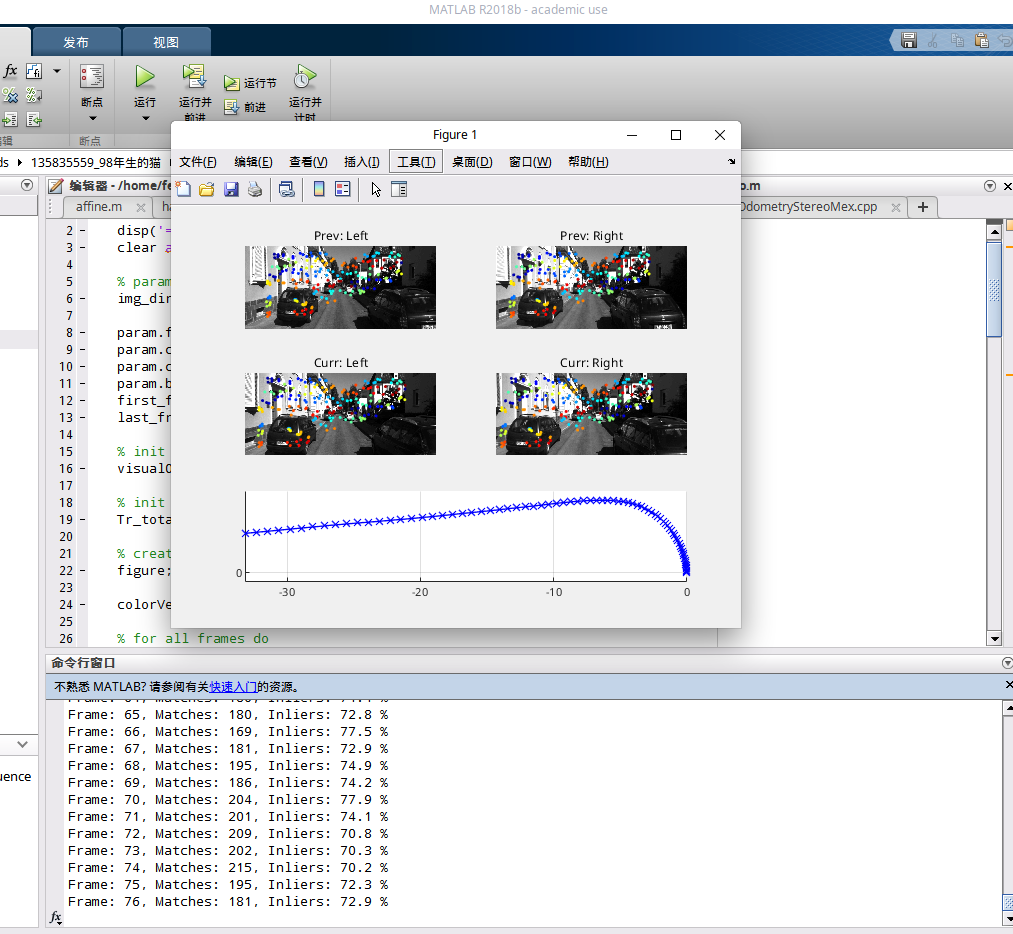
\includegraphics[width=0.8\textwidth]{img/matlab.png} 
        \caption{matlab版程序运行结果}
        \label{fig.4}
    \end{figure}
    程序试试显示当前匹配点的数量,inlier的比例,和主体的运动轨迹
    \subsection{c++版本}
    使用cmake生成makefile,通过make进行编译,然后下载官网上的demo进行测试,结果如图5
    \begin{figure}[H]
        \centering
        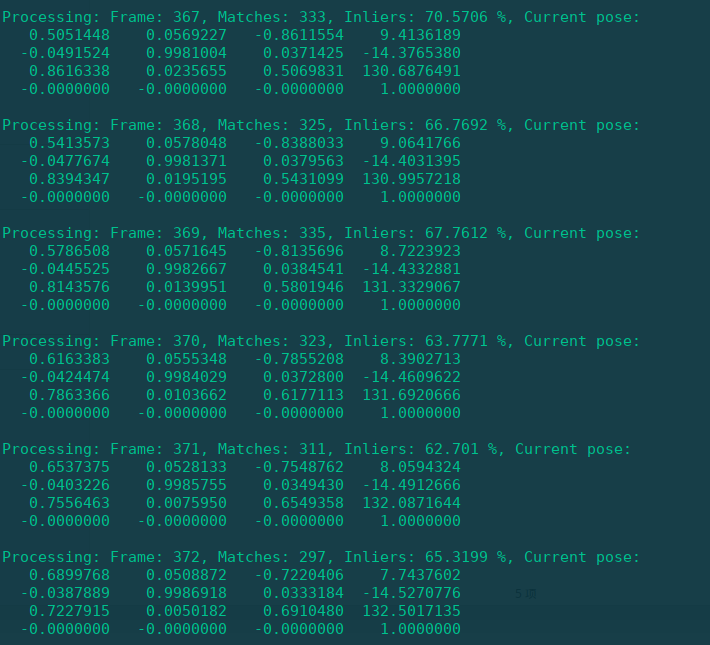
\includegraphics[width=0.6\textwidth]{img/c++.png} 
        \caption{c++版程序运行的结果}
        \label{fig.5}
    \end{figure}
    输出的结果与matlab版本相似,但是会直接输出位置矩阵,不会输出轨迹
\end{document}